W celu rozpoznania całego logo oparto się na identyfikacji cech wyznaczonych segmentów składowych: jednego czerwonego, żółtego i zielonego. By to osiągnąć skorzystano z parametrów, które w trakcie analizy dawały najbardziej charakterystyczne dla danych segmentów wyniki. Wybrano: niezmienniki momentowe \emph{NM1} i \emph{NM7} oraz współczynnik \emph{W3}  - Malinowskiej, którego wzór wygląda następująco:
\begin{equation}
    W3=\frac{L}{2\sqrt{\pi}S}-1
\end{equation}
\begin{center}
    gdzie $L$ - obwód segmentu, $S$ - jego pole.
\end{center}

Dla każdego z nich metodą eksperymentalną wyznaczono przedziały wartości - przedstawione w Tab.. Segment, którego wszystkie wartości współczynników będą należały do tych przedziałów zostanie zaklasyfikowany jako prawdopodobny segment składowy identyfikowanego logo (Rys. \ref{fig:segmenty_kolorow_poszczegolnych}).

\begin{table}[H]
    \centering
    \begin{tabular}{|c|c|c|c|}
    \hline
         Segment & NM1 & NM7 & W3 \\
         \hline
         czerwony & $[0,21, 0,28]$ & $[0,011, 0,014]$ &  $[0,66, 1,85]$\\
         \hline
         żółty & $[0,18, 0,38]$ & $[0,005, 0,022]$ &  $[0,75, 1,75]$\\
         \hline
         zielony & $[0,18, 0,34]$ & $[0,007, 0,12]$ &  $[0,45, 2,51]$\\
         \hline
    \end{tabular}
    \caption{Przedziały wartości wybranych współczynników charakterystycznych dla segmentów składowych logo}
    \label{tab:przedzialy_wspolczynnikow}
\end{table}

\begin{figure}[H]
\centering
\begin{subfigure}{.3\textwidth}
  \centering
  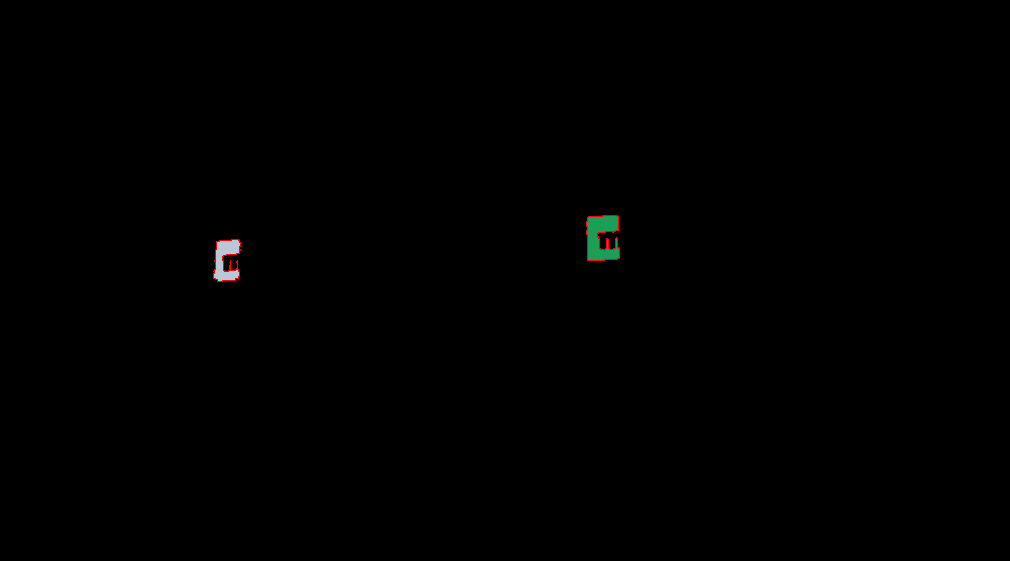
\includegraphics[width=.8\linewidth]{figures/img4_thresh_colored_red.png}
  \caption{Czerwony}
  \label{fig:sfig1}
\end{subfigure}
\begin{subfigure}{.3\textwidth}
  \centering
  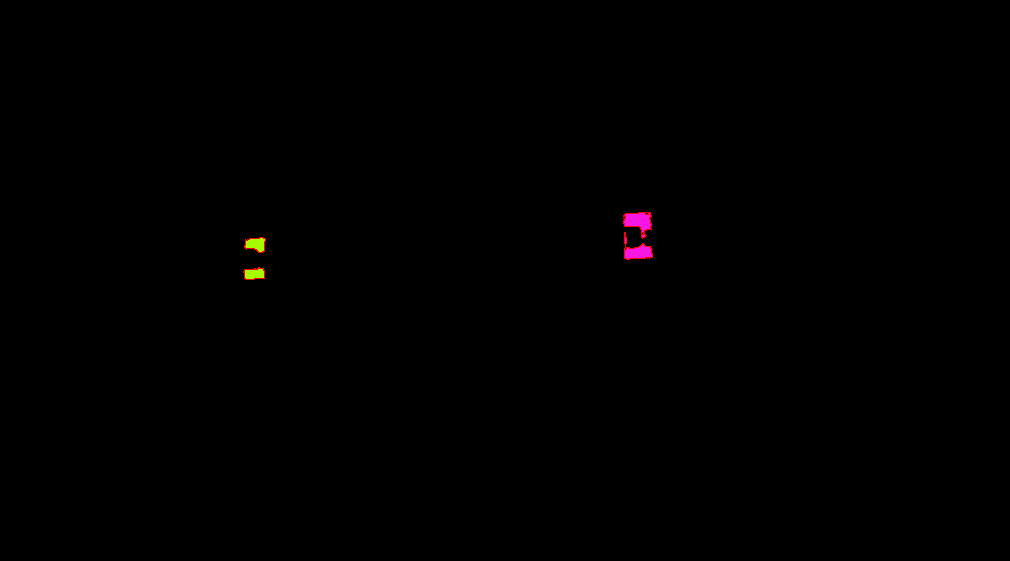
\includegraphics[width=.8\linewidth]{figures/img4_thresh_colored_yellow.png}
  \caption{Żółty}
  \label{fig:sfig2}
\end{subfigure}
\begin{subfigure}{.3\textwidth}
  \centering
  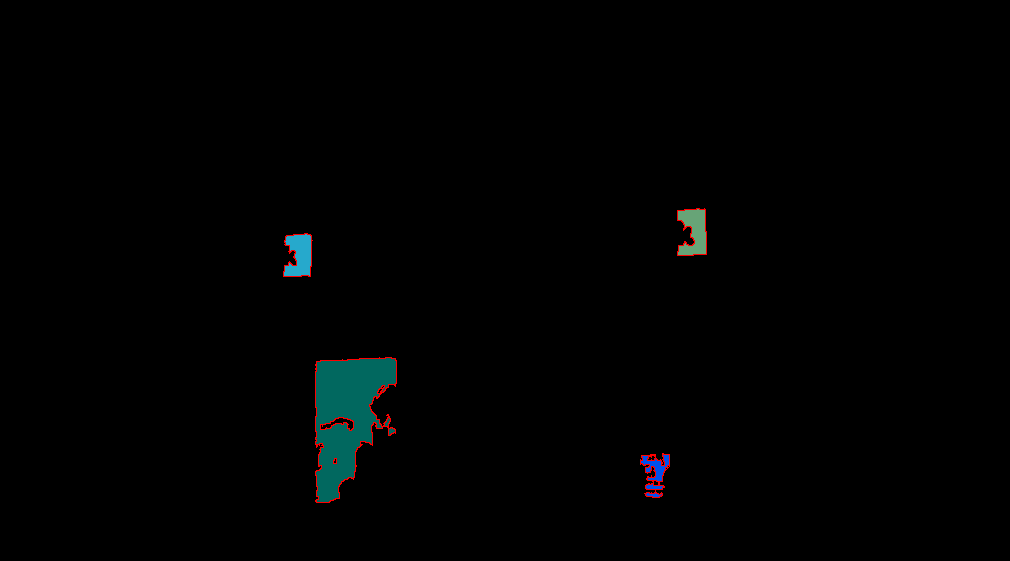
\includegraphics[width=.8\linewidth]{figures/img4_thresh_colored_green.png}
  \caption{Zielony}
  \label{fig:sfig2}
\end{subfigure}
\caption{Zaznaczone zidentyfikowane segmenty na obrazie \empty{d} dla poszczególnych kolorów}
\label{fig:segmenty_kolorow_poszczegolnych}
\end{figure}

Ostatecznym krokiem to identyfikacji samego logo jest przeszukanie kolekcji wszystkich wykrytych 3 typów segmentów i określenie położenia logotypu na podstawie względnego położenia 3 typów segmentów. Wykonywane jest to przy pomocy metody \textit{LogoRecognizer::findLogos}, a kryterium poprawnego zaklasyfikowania 3 segmentów jako składowe jednego logo jest wzajemna bliskość ich geometrycznych środków przy współczynniku $1,5$, określającym mnożnik długości przekątnej prostokąta opisanego na segmencie, który następnie traktowany jest jako promień koła wyznaczającego obszar sąsiedztwa danego segmentu. Tak pogrupowane segmenty są następnie łączone w jeden, który reprezentuje faktyczne zidentyfikowane logo (Rys. \ref{fig:segmenty_wszystkich_kolorow}).

\begin{figure}[H]
    \centering
    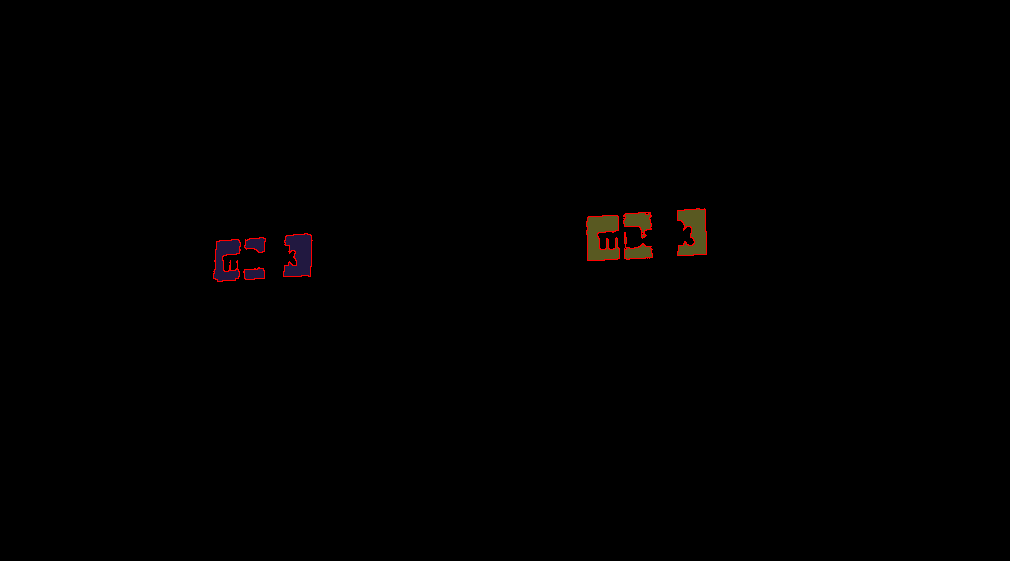
\includegraphics[width=10cm]{figures/img4_thresh_all_colored.png}
    \caption{Oznaczone segmenty połączone w jeden określający faktyczne zidentyfikowane logo}
    \label{fig:segmenty_wszystkich_kolorow}
\end{figure}
